\section{interaction overview diagram}

\subsection{Introduction}

\begin{flushleft}
La réalisation de mon interaction overview diagram s'est faite sur base de mon use case diagram. 
\end{flushleft}

\begin{flushleft}
Ce qui m'a permis encore une fois, de détailler la structure de ce diagramme intuitivement de la même manière que nous l'avions fait pour la base du projet.
\end{flushleft}

\begin{flushleft}
Nous allons donc repasser ensemble sur le nouveau parcours 
s'offrant au client.
\end{flushleft}

\begin{flushleft}
Notamment pour la gestion de portefeuilles et de consommations suite aux nouvelles permissions et possibilités lui étant 
octroyées.
\end{flushleft}

\newpage

\subsection{Accès à l'application pour les clients}

\begin{flushleft}
Lorsqu’un client \textbf{« gestionnaire »} voudra \textbf{voir ses portefeuilles} à partir du menu, il retrouvera plusieurs fonctionnalités :
\end{flushleft}

\begin{enumerate}[1.]
\item Créer portefeuille
\item Fermer un portefeuille
\item Visualisation des données de consommation
\item Gérer les données
\item Voir les utilisateurs invités
\end{enumerate}

\begin{flushleft}
Les quatre premières options étant identiques à la base, ne repassons pas sur ces dernières.
\end{flushleft}

\begin{flushleft}
Cependant, nous pouvons noter que l’\textbf{accès} à l’option « gérer les données » ne sera \textbf{jamais refusée} puisque le client est « gestionnaire » et maître de ses portefeuilles dans ce cas.
\end{flushleft}

\begin{enumerate}[-]
\item \textbf{Voir les utilisateurs invités : }
\end{enumerate}

\begin{enumerate}[a)]
\item Ajouter des utilisateurs
\item Supprimer des utilisateurs
\item Gérer les permissions
\end{enumerate}

\begin{enumerate}[-]

\item \textbf{Ajouter des utilisateurs :}

Le client « gestionnaire » se retrouvera alors sur une page où il pourra rechercher l’utilisateur qu’il souhaite inviter et ainsi, il pourra l’ajouter en inscrivant les permissions qu’il désire lui associer (lecture ou lecture et écriture).

\item \textbf{Supprimer des utilisateurs :}

Cela lui donnera la possibilité de supprimer un utilisateur invité s’il trouve cela plus judicieux.

\item \textbf{Gérer les permissions :}

Le gestionnaire aura la capacité de permettre une lecture seule ou une lecture et écriture à l’utilisateur invité.
\newline
\textbf{La lecture seule} comme son nom l’indique, permettra à ce dernier une « visualisation des données de consommation » et \textbf{la lecture et écriture} autorisera en plus de cela, de « gérer les données ».
\newline
L’ajout et la suppression d'utilisateurs ainsi que la gestion des permissions concernant les utilisateurs entraîneront \textbf{une notification} sur l’application des autres clients concernés.

\end{enumerate}

\newpage

\begin{flushleft}
Le menu offre désormais également la possibilité au client de \textbf{voir les portefeuilles où il est invité}, le client sera donc en mesure de :
\end{flushleft}

\begin{enumerate}[1.]
\item Voir des données de consommation
\item Gérer les données
\item Quitter un portefeuille
\end{enumerate}

\begin{enumerate}[-]
\item \textbf{Visualisation des données de consommation} :

\textbf{En cas de lecture seule}, le client pourra voir les données de consommation et donc garder un œil sur la gestion du portefeuille.

\item \textbf{Gérer les données :}

\textbf{En cas de lecture et écriture,} ce dernier aura la capacité de voir les données de consommation d’un portefeuille et de les modifier.
\newline
Si les \textbf{permissions} du client ne sont \textbf{pas valides}, autrement dit, le client n’a pas accès à la lecture et à l’écriture dans le portefeuille, alors, l’\textbf{accès} lui sera \textbf{refusé}.

\item \textbf{Quitter un portefeuille :}

Cela lui donnera la possibilité de quitter un portefeuille s’il trouve cela plus approprié.
\newline
Ce qui entraînera une \textbf{notification} du côté du client « \textbf{gestionnaire} ».

\end{enumerate}


\begin{figure}[h]
\subsection{Diagramme}
\centering
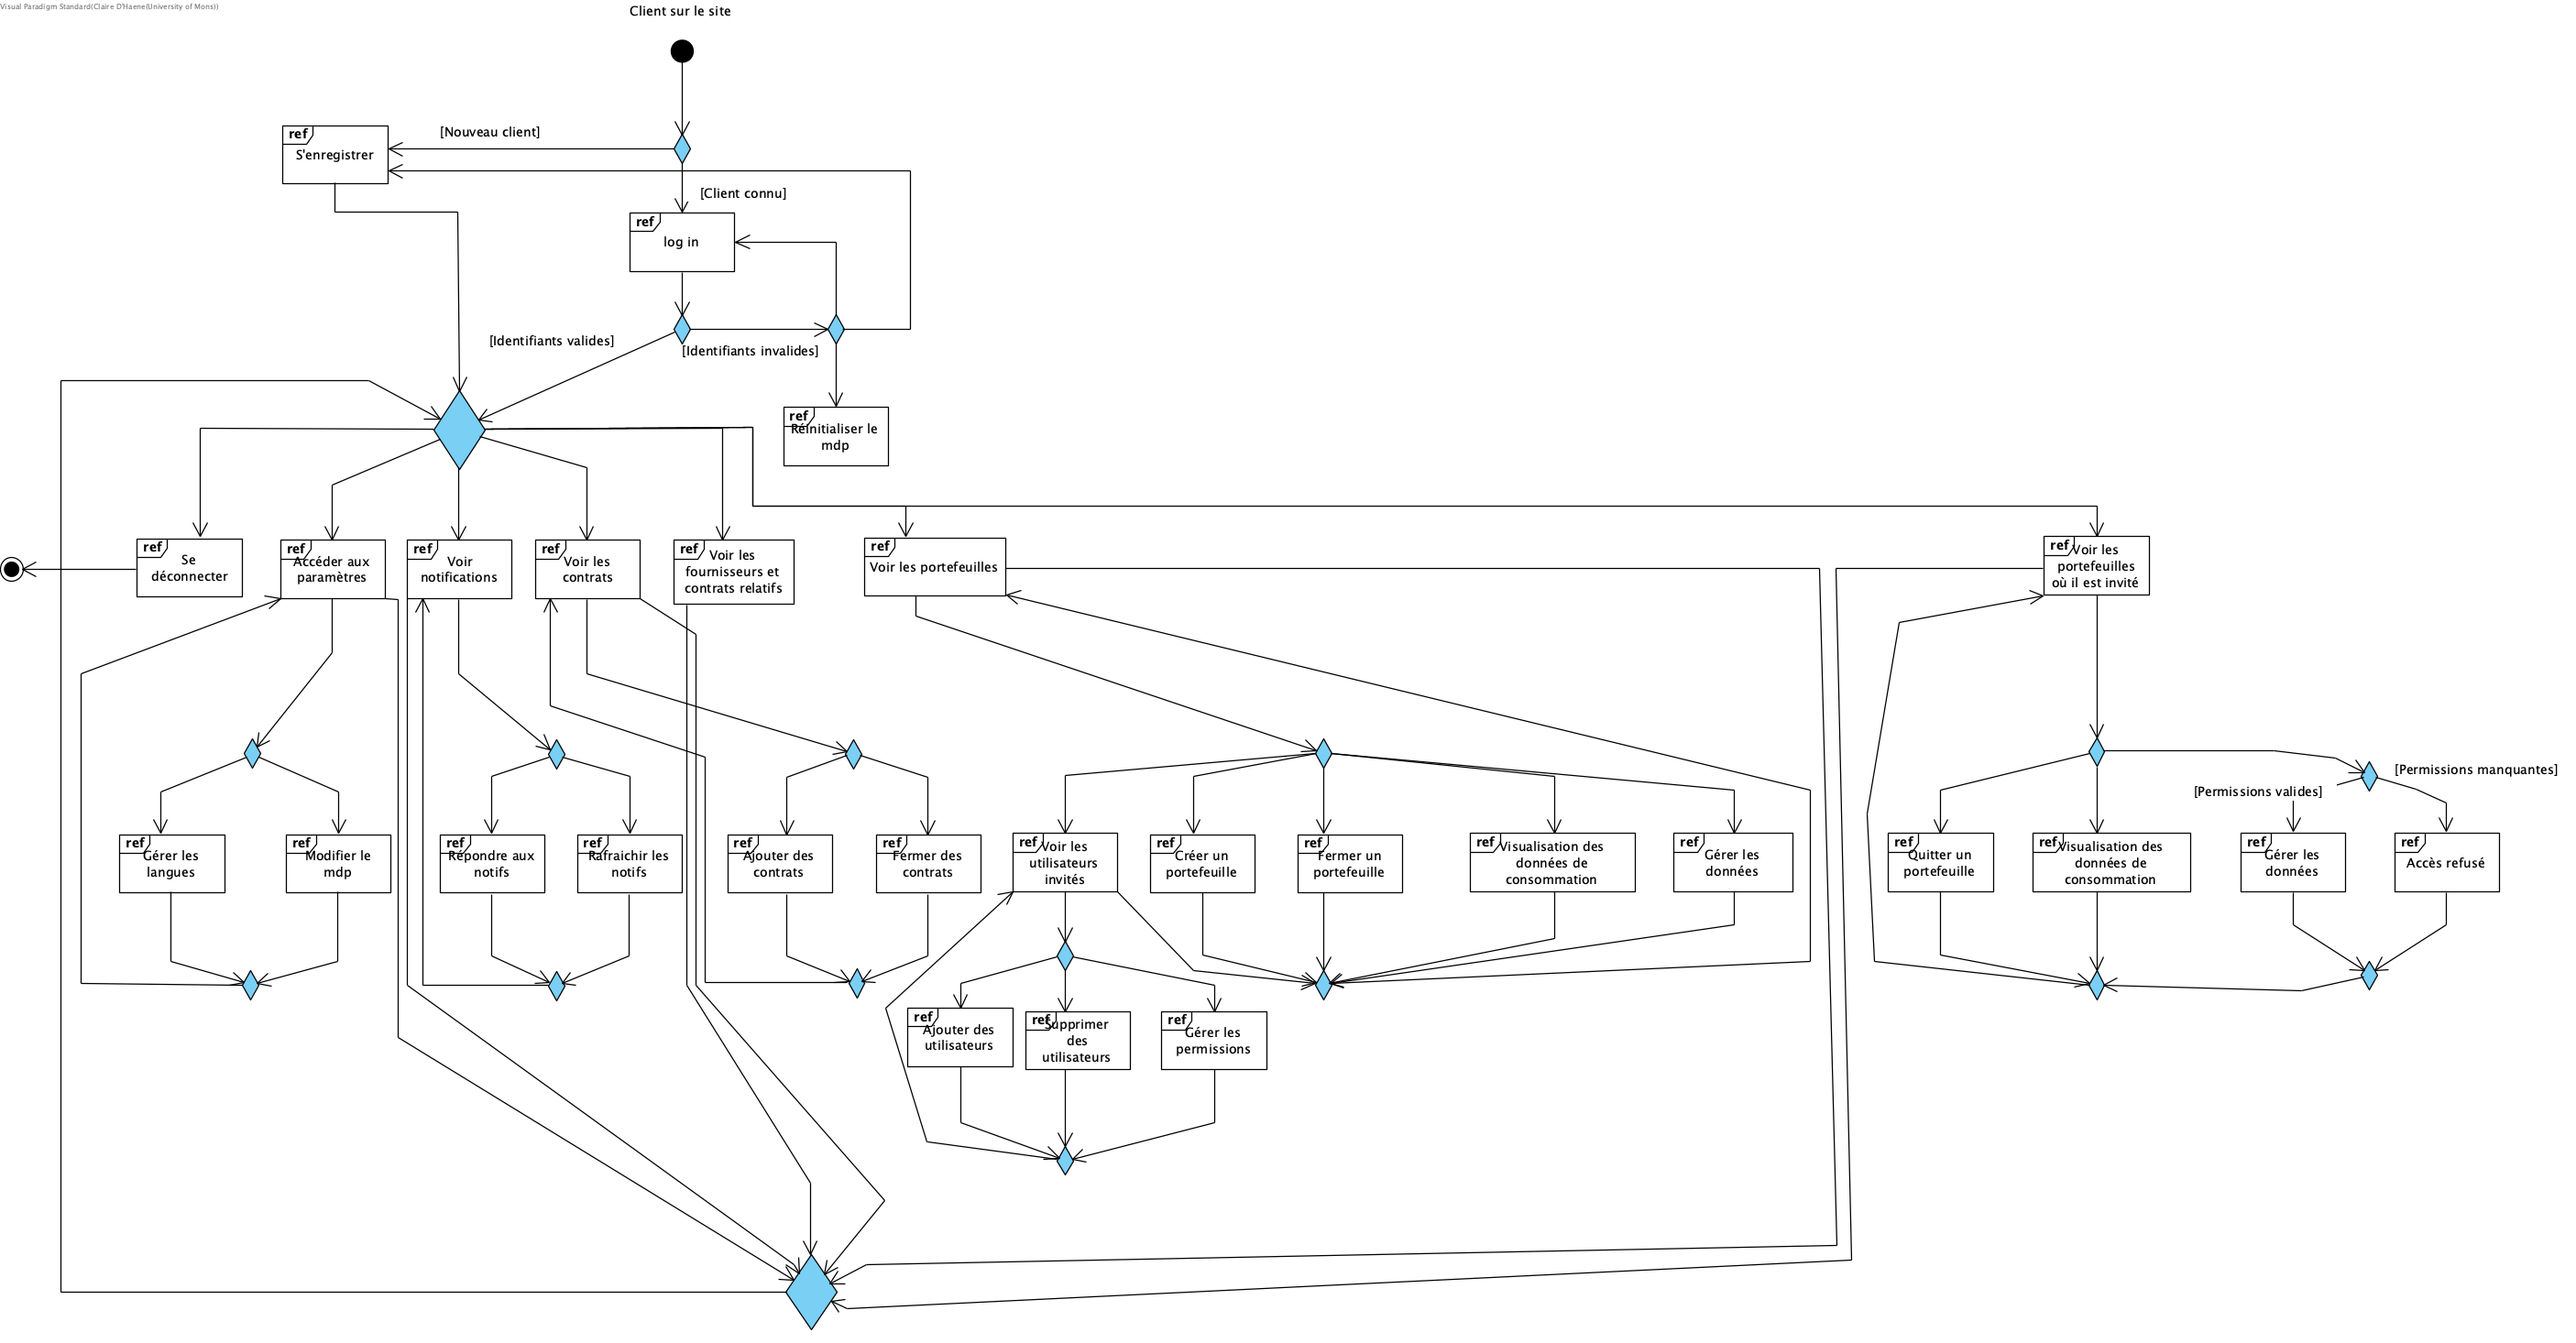
\includegraphics[width = 1\textwidth]{Extension-claire/Overview-claire/img/overview.png}
\end{figure}